\documentclass{l4dc2026}
\usepackage{times,booktabs,mathtools,float}
\jmlryear{2027}
\jmlrvolume{}
\jmlrproceedings{L4DC 2027}{L4DC 2027 research manuscript}
\title[Safe Holds and Actuator Identification]{When Safe Holds Hide Actuator Gains:\\Exact Resolution-Constrained Observation Scheduling}
\author{\Name{Shivam Gupta} \Email{shivam1720406@gmail.com}\\\addr Independent Researcher}
\newcommand{\R}{\mathbb{R}}
\newcommand{\W}{\mathcal{W}}
\newcommand{\X}{\mathcal{X}}
\newcommand{\U}{\mathcal{U}}
\newcommand{\norm}[1]{\left\lVert #1\right\rVert}
\newcommand{\diam}{\operatorname{diam}}
\newcommand{\supp}{\operatorname{supp}}
\newcommand{\gauge}{\gamma}
\begin{document}
\raggedbottom
\maketitle
\begin{abstract}
Self-triggered controllers choose when to observe again, but a safe observation interval need not be an informative one. We study endpoint-only identification of a constant scalar actuator gain under held inputs, known linear state dynamics, and bounded process disturbances. We characterize the exact worst-case diameter of the next feasible parameter interval using the gauge of the accumulated disturbance set. Combining this characterization with exact robust prefix constraints gives a finite, globally solved duration--resolution frontier. A family of strictly stable oscillators exhibits an unbounded ratio between the resolution scores of one-step and full-period holds, even when both are safe. We also establish a disturbance-induced ambiguity floor that arbitrary adaptive sampling cannot remove. For scaled orthogonal dynamics and Euclidean bounds, all calculations reduce to scalar interval intersections. A reproducible study of 2,400 simulated episodes compares six scheduling rules across four plants and two disturbance regimes. In the two oscillatory plants, a short informative probe followed by long holds resolves the gain with 11 observations, whereas the longest-hold rule uses 10 observations without reaching the target. Nonoscillatory and mixed-mode controls delimit the effect. Independent numerical checks and a model-error experiment test the certificates and their assumptions.
\end{abstract}
\begin{keywords}
Safe system identification; self-triggered control; bounded-error experiment design; observation scheduling; actuator uncertainty.
\end{keywords}

\section{Introduction}
A networked actuator can continue executing a command while its supervisor sleeps. The next observation then serves two purposes: checking the physical state and learning how the actuator responds. These purposes do not impose the same timing requirements. A command can remain safe for many steps while its accumulated effect nearly cancels at the observation time. Extending a safe hold may therefore save telemetry precisely by removing the evidence needed for actuator calibration.

Remote commissioning motivates jointly reducing telemetry and learning an actuator model. Industrial wireless systems must account for time, reliability, energy, and scale \citep{nist}. Self-triggered control selects execution times from the current state \citep{anta2010}, and adaptive variants already combine aperiodic observations with safe learning \citep{zhang2019,dhiman2022}. We ask: \emph{what parameter resolution can a safe held command guarantee from its endpoint alone?}

The distinction can be sharp even for a known, strictly stable state matrix. Let $A=aR_{2\pi/H}$ be a damped planar rotation and let an unknown gain multiply a constant input direction $c$. The gain's endpoint sensitivity is $q_h=\sum_{i=0}^{h-1}A^i c$. Intermediate states may remain safe although $q_H$ is small. For $a=1$, the full-period sensitivity vanishes exactly. For $a<1$, identification is possible in principle, but its worst-case resolution deteriorates without bound relative to a one-step hold as $a$ approaches one. This is an excitation cancellation mechanism in an already discrete model, rather than a claim about reconstructing continuous-time frequencies above Nyquist.

We characterize the sharp next-observation diameter for symmetric disturbance sets and solve its state-dependent safe duration frontier. A stable cancellation family shows an unbounded loss in normalized resolution. A short-probe remedy reaches minimax-optimal resolution using at most one extra endpoint. Closed-form implementation permits independent checks and controlled comparisons in which all rules share safety constraints and parameter updates.

\section{Related work and scope of the contribution}
\paragraph{Safe intermittent learning.}
\citet{zhang2019} construct a zonotope-based estimator compatible with aperiodic sampling and use uncertainty in a self-triggered min--max MPC scheduler. \citet{dhiman2022} learn control-affine dynamics with matrix-variate Gaussian processes and synthesize probabilistically safe self-triggered controls. Robust CBF methods can reduce actuation uncertainty online through integral set-membership identification \citep{cohen2022}. Predictive safety filters certify learning-based inputs through constrained prediction \citep{wabersich2021}. The present work does not replace these frameworks or claim their learning components are unsound. It supplies an explicit resolution constraint for a restricted endpoint-only experiment and examines what a duration objective can omit.

\paragraph{Bounded-error experiment design.}
Set-membership identification retains all compatible parameters \citep{kosut1992}; optimizing their set size is established \citep{pronzato1990}. \citet{tanaskovic2014} characterize optimal worst-case experiments with general linear regressors and convex input constraints. Optimal scalar-gain designs also exist for binary and quantized sensors \citep{casini2011,casini2012}. Bounded-error sampling design includes nonlinear applications \citep{marvel2012} and constrained min--max methods \citep{walz2018}. Our narrower problem combines held commands, integer observation gaps, duration-dependent accumulated process disturbances, and robust state constraints on every unobserved prefix. The resulting scalar frontier specializes established worst-case geometry; maximal-amplitude probing itself is not a new principle.

\paragraph{Sampling and excitation.}
\citet{gonzalez2024} analyze statistical identification under slow sampling; \citet{dozzi2026} optimize nonuniform sampling for multisine identification. Sampling-dependent informativeness is therefore not itself new. Here the known discrete matrix and unknown scalar gain yield a held-input regressor whose cancellation can be quantified under prefix safety. The contribution is this characterization and evaluation, rather than a universal learning controller.

\section{Endpoint-only experiments and exact safety}
Consider the discrete-time system
\begin{equation}\label{eq:model}
 x_{t+1}=Ax_t+\theta c u_t+w_t,\qquad
 \theta\in\Theta=[\ell,r],\quad w_t\in\W,\quad |u_t|\le U.
\end{equation}
The matrix $A\in\R^{n\times n}$ and direction $c\ne0$ are known. The gain $\theta$ is unknown and constant. The compact convex set $\W$ is centrally symmetric about zero and has nonempty interior. Disturbances can be arbitrary and policy-dependent within $\W$; independence or zero mean is not assumed. At an observation time the state $x$ is measured exactly. The supervisor selects $(u,h)$, holds $u$ for $h$ steps, and receives only $y=x_{t+h}$. States must lie in a closed convex safe set $\X$ at every integer time, including unobserved times. Continuous-time motion between these times is outside the model.

Define
\begin{equation}\label{eq:lift}
 q_j=\sum_{i=0}^{j-1}A^i c,\qquad
 \W_j=\bigoplus_{i=0}^{j-1}A^i\W,\qquad
 x_{t+j}\in A^jx+\theta q_j u+\W_j.
\end{equation}
This reachable set is exact at each prefix: every member of $\W_j$ corresponds to admissible step disturbances. The same $\theta$ is used throughout a hold. The support function is $s_C(v)=\sup_{z\in C}v^\top z$, and the gauge is $\gauge_C(v)=\inf\{\lambda\ge0:v\in\lambda C\}$.

\begin{lemma}[Exact prefix-safe inputs]\label{lem:safe}
Define $I_h(x,\Theta)$ as the set of $u\in[-U,U]$ satisfying
\begin{equation}\label{eq:safe}
 A^jx+\theta q_j u+\W_j\subseteq\X
 \quad(j=1,\ldots,h;\ \theta\in\{\ell,r\}).
\end{equation}
Then $I_h$ is a closed interval, possibly empty, nested as $I_{h+1}\subseteq I_h$. Equation~\eqref{eq:safe}, together with $|u|\le U$, is necessary and sufficient for robust safety during the hold. If $\X=\{z:Fz\le b\}$, it is equivalent to the scalar linear inequalities
\begin{equation}\label{eq:poly}
 F_k A^jx+\theta F_kq_j u+\sum_{i=0}^{j-1}s_\W((A^i)^\top F_k^\top)\le b_k.
\end{equation}
\end{lemma}
\begin{proof}
The dependence on $\theta$ is affine; each intermediate parameter is a convex combination of the endpoint reachable sets. Convexity of $\X$ therefore makes the two endpoint tests sufficient. Necessity follows by choosing an endpoint parameter and a disturbance sequence attaining a violating reachable point. Each inclusion is convex in scalar $u$, so their intersection with $[-U,U]$ is an interval. Additional prefixes only add constraints. Support functions of Minkowski sums add, yielding~\eqref{eq:poly}.
\end{proof}

Finite-hold safety alone does not establish indefinite feasibility. One can additionally impose a terminal inclusion in a robust control-invariant subset $K\subseteq\X$. Alternatively, if $A\X\oplus\W\subseteq\X$, the zero input is a safe backup. Our experiments use the latter condition, making every duration feasible at least at $u=0$ and avoiding a hidden terminal-feasibility assumption.

\section{Exact resolution and the duration frontier}
The endpoint feasible parameter set is
\begin{equation}\label{eq:post}
 \Theta^+(y;u,h)=\{\vartheta\in\Theta:y-A^h x-\vartheta q_hu\in\W_h\}.
\end{equation}
It is an interval and contains the true parameter for every admissible disturbance. Write $D=r-\ell$ and adopt $2/0=+\infty$.

\begin{theorem}[Sharp next-observation diameter]\label{thm:diam}
For any fixed feasible $(u,h)$,
\begin{equation}\label{eq:diam}
 \sup_{y:\Theta^+(y;u,h)\ne\varnothing}\diam\Theta^+(y;u,h)
 =d(u,h;\Theta):=\min\left\{D,\frac{2}{|u|\gauge_{\W_h}(q_h)}\right\}.
\end{equation}
The supremum is attained by the noiseless endpoint of the prior midpoint. Consequently $d/2$ is the minimax absolute-error radius for estimating the gain from this one endpoint.
\end{theorem}
\begin{proof}
If $\vartheta_1,\vartheta_2$ are compatible with the same endpoint, subtracting their residuals gives
$(\vartheta_1-\vartheta_2)q_hu\in\W_h-\W_h=2\W_h$.
Thus their distance is at most $2/(|u|\gauge_{\W_h}(q_h))$, and it is also at most $D$. Let $m=(\ell+r)/2$ and choose $y=A^hx+m q_hu$. Compatibility is then exactly
$|\vartheta-m|\,|u|\gauge_{\W_h}(q_h)\le1$.
Its intersection with the centered prior attains the stated diameter. This endpoint is realizable with $\theta=m$ and zero disturbance. The midpoint of any compatible interval has maximal absolute error half its width; the two compatible endpoints force that radius for any estimator.
\end{proof}



\begin{theorem}[Exact conditional frontier]\label{thm:frontier}
For every nonempty $I_h$, let $M_h=\max_{u\in I_h}|u|$ and $\kappa_h=\gauge_{\W_h}(q_h)$. The minimum worst-case next-observation diameter at duration $h$ is
\begin{equation}\label{eq:dh}
 d_h^*=\min\{D,2/(M_h\kappa_h)\}.
\end{equation}
For a target $0<\delta<D$ and $h\in\{1,\ldots,H_{\max}\}$, the largest duration guaranteeing diameter at most $\delta$ is exactly
\begin{equation}\label{eq:rcd}
 h^*=\max\{h:I_h\ne\varnothing,\ M_h\kappa_h\ge2/\delta\}.
\end{equation}
If the set is empty, no admissible held input in the duration menu can guarantee the target from the next endpoint.
\end{theorem}
\begin{proof}
Equation~\eqref{eq:diam} is nonincreasing in $|u|$. On a compact interval the maximum magnitude is attained at one of its endpoints. Substituting this value gives~\eqref{eq:dh}; rearranging the diameter condition gives~\eqref{eq:rcd}. Finite enumeration proves global optimality within the stated menu and held-input class.
\end{proof}

We call the rule in~\eqref{eq:rcd} \emph{resolution-constrained dwell} (RCD). When $D\le\delta$, it selects the longest feasible duration. If the target is infeasible, our implementation selects a duration minimizing $d_h^*$, breaking ties toward longer holds. It uses the largest-magnitude safe input, with a positive-input tie break. This choice isolates identification; it does not minimize control effort or tracking error. A performance controller could instead optimize over
$I_h\cap\{u:|u|\ge2/(\delta\kappa_h)\}$, the union of at most two intervals. RCD is optimal for the \emph{conditional next-observation} problem, not for a finite-horizon trajectory of future observations. In particular, a shorter initial probe can enable long holds sooner.



\section{Cancellation and limits to learning}
\begin{theorem}[Safe full-period holds can be arbitrarily less informative]\label{thm:cancel}
Let $A=aR_{\phi}$, $\phi=2\pi/H$, $H\ge3$, $0<a<1$, $\norm{c}=1$, and $\W=\eta\mathbb B_2$ with $\eta>0$. Let $g_h=\norm{q_h}/\sum_{i=0}^{h-1}a^i$, so $\kappa_h=g_h/\eta$. Then
\begin{equation}\label{eq:cancel}
 g_1=1,\qquad
 g_H=\frac{1-a}{|1-ae^{\mathrm i\phi}|},\qquad
 \frac{g_1}{g_H}\longrightarrow+\infty\quad\text{as }a\uparrow1.
\end{equation}
There exist safe balls, containing the origin, for which $u=U$ is safe for every $h\le H$ and zero is an invariant backup. Hence safety does not bound the ratio in~\eqref{eq:cancel}. At $a=1,\eta=0$, a full-period hold has zero gain sensitivity, while any nonzero hold of length $H-1$ identifies the scalar gain exactly.
\end{theorem}
\begin{proof}
Identify the plane with the complex numbers, taking $c=1$ without loss of generality. Then
$q_h=(1-(ae^{\mathrm i\phi})^h)/(1-ae^{\mathrm i\phi})$.
For $h=H$, its magnitude is $(1-a^H)/|1-ae^{\mathrm i\phi}|$, whereas $\sum_{i=0}^{H-1}a^i=(1-a^H)/(1-a)$. This proves the formula and its limit. For a bounded prior choose the safe radius at least
$\max\{\eta/(1-a),\max_{j\le H}[\max(|\ell|,|r|)U\norm{q_j}+\eta\sum_{i<j}a^i]\}$.
Starting at zero, every stated input prefix is then safe; $aR+\eta\le R$ proves zero-input invariance. For $a=1$, geometric summation yields $q_H=0$ and $q_{H-1}\ne0$. With no disturbance, a nonzero regressor determines the gain from one endpoint.
\end{proof}
The safe radius may grow along the limiting family. The theorem establishes a separation, not an unbounded effect in one fixed physical device. For any selected stable member the radius is finite. Cancellation also persists under small detuning because the finite sum defining $q_h$ is continuous in $a$ and $\phi$; exact periodicity is unnecessary for a large finite gap.

\begin{figure}[H]
\centering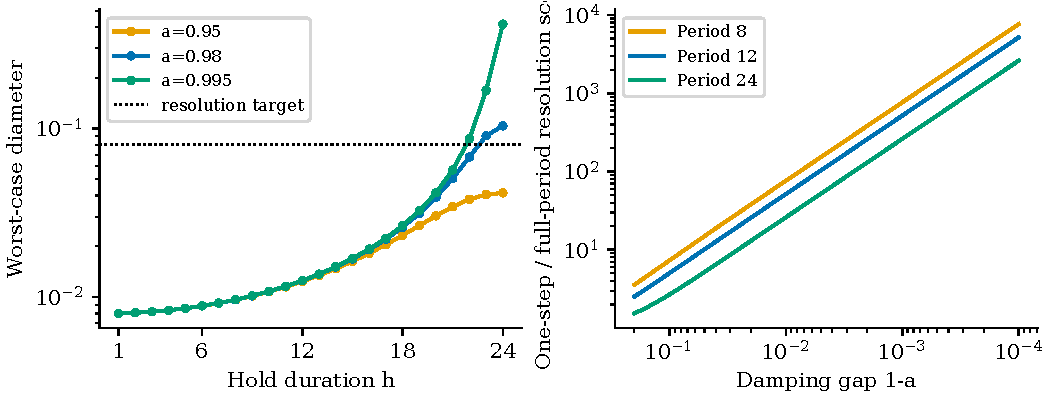
\includegraphics[width=.98\linewidth]{figures/mechanism.pdf}
\caption{Endpoint cancellation under bounded per-step noise. Left: worst-case diameter at fixed input $.25$ and period 24, for three strictly stable damping factors. Right: the exact one-step/full-period score ratio from~\eqref{eq:cancel}. The diameter is clipped by the prior width; the score ratio is not.}\label{fig:mechanism}
\end{figure}

No hold exceeds the one-step normalized worst-case information ceiling per unit input in this disturbance model; information can behave differently under a stochastic model.
\begin{proposition}[Resolution ceiling and ambiguity floor]\label{prop:floor}
For the general model~\eqref{eq:model},
\begin{equation}\label{eq:ceiling}
 \gauge_{\W_h}(q_h)\le\gauge_\W(c).
\end{equation}
For any adaptive input and observation policy with $|u_t|\le U$, there exist two gains in the prior, separated by
\begin{equation}\label{eq:floor}
 d_0=\min\{D,2/(U\gauge_\W(c))\},
\end{equation}
and admissible disturbance sequences producing identical complete state trajectories. Thus arbitrary sampling cannot guarantee gain error below $d_0/2$ on this model class.
\end{proposition}
\begin{proof}
Put $g=\gauge_\W(c)$. Since $c\in g\W$, summation gives $q_h\in g\W_h$, proving~\eqref{eq:ceiling}. Choose $\theta_\pm=m\pm d_0/2$ with prior midpoint $m$. Under either gain set $w_t=(m-\theta_\pm)c u_t$. Its gauge is at most $d_0U g/2\le1$. Both systems therefore follow $x_{t+1}=Ax_t+mcu_t$. Identical observations generate identical subsequent choices by induction; a common random seed couples randomized policies too. Any estimate incurs error at least $d_0/2$ in one compatible system.
\end{proof}
\begin{corollary}[Optimal resolution with at most one extra observation]\label{cor:packet}
Suppose $A=aQ$, $Q$ is orthogonal, $\W=\eta\mathbb B_2$, and zero input keeps $\X$ invariant. If a one-step input of magnitude $U$ is robustly safe at the initial state, one endpoint achieves the optimal worst-case diameter
\[
 d_0=\min\{D,2\eta/(U\norm{c})\}.
\]
For an episode of $T$ steps in a protocol requiring an endpoint after each hold of at most $H_{\max}$ steps, this resolution and robust safety can be maintained using
\[
 N=1+\left\lceil\frac{T-1}{H_{\max}}\right\rceil
 \le\left\lceil\frac{T}{H_{\max}}\right\rceil+1
\]
observations, including the final endpoint. Any such protocol requires at least $\lceil T/H_{\max}\rceil$ observations.
\end{corollary}
\begin{proof}
At one step, $q_1=c$ and $\rho_1=\eta$, so Theorem~\ref{thm:diam} gives $d_0$; Proposition~\ref{prop:floor} rules out a smaller uniform diameter after any number of observations. Use zero-input holds for the remaining steps, truncating the last hold. Safety follows by invariance and subsequent intersections cannot enlarge the gain interval. The count follows by partitioning $T-1$ steps into holds of length at most $H_{\max}$; the lower bound follows from the same duration cap.
\end{proof}
This statement formalizes a simple remedy, not a need for a complex scheduler. The full-amplitude safe-probe assumption can fail near a constraint boundary; the state-dependent frontier then remains useful. The observation-count bound uses the stated endpoint-per-hold protocol: an actuator allowed to coast indefinitely without reporting has a different communication accounting.

This is the standard bounded-error indistinguishability mechanism specialized to gain learning. It prevents interpreting random-noise interval shrinkage as a distribution-free consistency guarantee. It also explains why the information proxy below is a comparator rather than a robust substitute: covariance-based information adds across independent random errors, while adversarial errors can persistently mimic a gain change.

\section{Closed-form implementation and robustness}
For $A=aQ$, $Q^\top Q=I$, $0<a<1$, $\W=\eta\mathbb B_2$, and $\X=R\mathbb B_2$, rotational symmetry gives
\begin{equation}\label{eq:rho}
 \W_j=\rho_j\mathbb B_2,\quad \rho_j=\eta\sum_{i<j}a^i,\quad
 \norm{A^jx+\theta q_ju}\le R-\rho_j\quad(\theta=\ell,r).
\end{equation}
Each inequality is a scalar quadratic sublevel set. Let $b=A^jx$, $v=\theta q_j$, and $s=R-\rho_j$. For $\norm{v}>0$ its interval has center and squared half-width
\begin{equation}\label{eq:quad}
 z=-\frac{b^\top v}{v^\top v},\qquad
 L^2=\frac{s^2-b^\top b}{v^\top v}+z^2.
\end{equation}
Negative $s$ or $L^2$ implies infeasibility; a zero $v$ requires $\norm{b}\le s$. Prefix intersections yield all $I_h$ in one pass after the lifted vectors have been computed. With $n$-dimensional states, cached powers require $O(H_{\max}n^2)$ storage, and each online evaluation requires $O(H_{\max}n^2)$ arithmetic using those powers. The two- and three-dimensional experiments use ordinary double precision, not interval-certified floating-point arithmetic.

The endpoint update is a closed-form line--ball intersection, given in Appendix~\ref{app:geometry}. Empty intersections are retained as model inconsistencies.

\paragraph{Known dynamics are a substantive assumption.}
If the true matrix is $A+E$ with $\norm{E}_2\le\varepsilon$, the residual $Ex_t$ can be treated as extra disturbance. Within $R\mathbb B_2$, replacing $\eta$ by $\eta_{\mathrm{eff}}=\eta+\varepsilon R$ in the nominal calculation is sound. A first-exit argument justifies this use of the state bound: until an exit all residuals satisfy the inflated bound, and the certificate rules out the exit. The resulting posterior contains the true gain, but its diameter formula is an outer-model guarantee, not an exact description of the fixed-$E$ problem. Recursive zero-input feasibility follows if $aR+\eta_{\mathrm{eff}}\le R$. Unknown disturbance magnitudes or unbounded observation errors require additional assumptions; they are not covered by the nominal certificates.

\section{Reproducible evaluation}
\paragraph{Protocol.}
The experiment plan was saved before the main simulations. Four known matrices are tested: planar rotations of periods 8 and 24 with damping $.98$ and $.995$, respectively; a nonoscillatory contraction $.94I_2$; and a three-dimensional matrix $.98\operatorname{diag}(R_{2\pi/12},1)$ with direction proportional to $(1,0,.3)$. All use $\eta=.001$, $R=1$, $U=.25$, $H_{\max}=24$, and prior $[.5,1.5]$. Fifty seeds per plant draw $\theta$ uniformly from $[.6,1.4]$ and an initial state uniformly in the radius-$.2$ ball. Each episode has 240 physical steps. The target diameter is $.08$. All plants satisfy $aR+\eta\le R$.

Six rules share exact safe intervals, maximal-magnitude inputs, and~\eqref{eq:inverse}: longest feasible hold; fixed hold at most six steps; one-step probing; minimax diameter with longer ties; a Gaussian-information proxy maximizing $u^2\norm{q_h}^2/\sum_{i<h}a^{2i}$; and RCD. These are controlled objective comparisons, not implementations of complete published MPC or GP controllers. The minimax rule automatically switches to long holds once the prior width clips every subsequent diameter bound. It therefore implements a simple resolve-then-hold behavior without an additional learned scheduler.

Random disturbances are independent uniform draws in the radius-$.001$ ball; all rules on a seed receive the same physical-time disturbance tape. The second regime constructs policy-dependent bounded disturbances that move each endpoint toward the current prior-midpoint response as far as its disturbance ball allows. It tests adversarial ambiguity, not expected performance or a common-noise paired comparison. There are $4\times50\times6\times2=2,400$ episodes and 576,000 physical transitions. The separate model-error extension uses 200 episodes; it was specified before its own run.

\paragraph{Results.}
Table~\ref{tab:main} reports all random-noise outcomes. On Rotation-8, longest holds leave mean diameter $.25136$; on Rotation-24 they leave $.60361$. Neither reaches the target in any seed. RCD yields $.00951$ and $.00914$ with 11 observations rather than 10. The paired RCD-minus-longest differences are $-.24185$ and $-.59446$, with bootstrap intervals $[-.24595,-.23771]$ and $[-.63753,-.55047]$. These use 20,000 paired resamples and 98.75\% marginal coverage, a Bonferroni allocation for the four declared plant comparisons. They describe this simulation distribution, not physical-device reliability.

\begin{table}[t]
\centering\small
\caption{Random disturbances: means over 50 seeds; diameter includes sample standard deviation. ``Time resolved'' is the fraction of physical steps whose most recently observed interval has width at most $.08$. All six rules are retained.}\label{tab:main}
\begin{tabular}{llrrr}
\toprule
Plant & Rule & Diameter & Observations & Time resolved \\
\midrule
rotation8 & Longest & $0.25136\pm0.01183$ & 10.0 & 0.000 \\
rotation8 & Fixed-6 & $0.01420\pm0.00179$ & 40.0 & 0.975 \\
rotation8 & One-step & $0.00006\pm0.00004$ & 240.0 & 0.996 \\
rotation8 & Minimax & $0.00699\pm0.00133$ & 11.0 & 0.996 \\
rotation8 & Gaussian proxy & $0.00290\pm0.00069$ & 80.0 & 0.987 \\
rotation8 & RCD & $0.00951\pm0.00062$ & 11.0 & 0.912 \\
\midrule
rotation24 & Longest & $0.60361\pm0.12532$ & 10.0 & 0.000 \\
rotation24 & Fixed-6 & $0.00525\pm0.00074$ & 40.0 & 0.975 \\
rotation24 & One-step & $0.00005\pm0.00003$ & 240.0 & 0.996 \\
rotation24 & Minimax & $0.00699\pm0.00133$ & 11.0 & 0.996 \\
rotation24 & Gaussian proxy & $0.00429\pm0.00096$ & 40.7 & 0.987 \\
rotation24 & RCD & $0.00914\pm0.00090$ & 11.0 & 0.924 \\
\midrule
nonoscillatory & Longest & $0.01698\pm0.00433$ & 10.0 & 0.900 \\
nonoscillatory & Fixed-6 & $0.00433\pm0.00056$ & 40.0 & 0.975 \\
nonoscillatory & One-step & $0.00005\pm0.00003$ & 240.0 & 0.996 \\
nonoscillatory & Minimax & $0.00759\pm0.00049$ & 11.0 & 0.990 \\
nonoscillatory & Gaussian proxy & $0.00477\pm0.00081$ & 30.2 & 0.987 \\
nonoscillatory & RCD & $0.01698\pm0.00433$ & 10.0 & 0.900 \\
\midrule
mixed3d & Longest & $0.02638\pm0.00447$ & 10.0 & 0.900 \\
mixed3d & Fixed-6 & $0.00704\pm0.00075$ & 40.0 & 0.975 \\
mixed3d & One-step & $0.00004\pm0.00003$ & 240.0 & 0.996 \\
mixed3d & Minimax & $0.00638\pm0.00141$ & 11.0 & 0.996 \\
mixed3d & Gaussian proxy & $0.00368\pm0.00112$ & 56.0 & 0.987 \\
mixed3d & RCD & $0.02638\pm0.00447$ & 10.0 & 0.900 \\
\bottomrule
\end{tabular}
\end{table}

The minimax rule is the stronger practical choice in the oscillatory cases: it reaches the target after one step in every seed and then uses long holds, also totaling 11 observations. RCD delays the initial observation to obtain a longer immediately certified hold; its average first target times are 21 and 18.2. Thus exact optimality for the next-observation frontier does not imply optimality for a commissioning episode. One-step probing achieves much narrower final intervals, approximately $5\times10^{-5}$, but uses 240 observations. The fixed-six and Gaussian-proxy rules occupy intermediate trade-offs. Figure~\ref{fig:comparison} makes the resource comparison explicit.

\begin{figure}[t]
\centering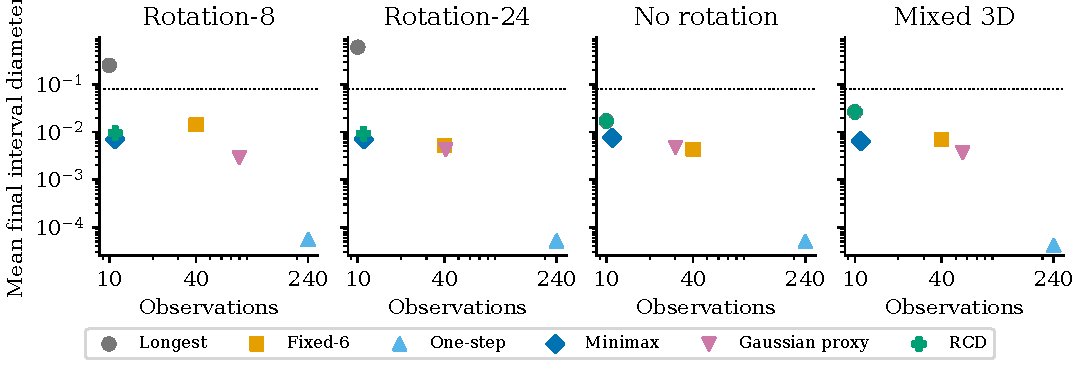
\includegraphics[width=\linewidth]{figures/comparison.pdf}
\caption{All random-noise rules: final uncertainty versus endpoint observation count, averaged over 50 seeds. Lower and left are preferable for these two metrics. RCD coincides with longest holds on the nonoscillatory and mixed-mode plants. A short minimax probe followed by long holds performs well here; universal dominance is not claimed.}\label{fig:comparison}
\end{figure}

On the nonoscillatory and mixed-mode controls, RCD and longest holds produce identical runs, with final diameters $.01698$ and $.02638$. The extra fixed-axis component in the latter preserves endpoint sensitivity when the rotating component cancels. This negative control limits the result: long holds are not inherently uninformative. Under the adversarial regime, the longest-hold oscillatory diameters increase to $.30318$ and $.88514$, whereas the minimax rule stops at the predicted $.008$ floor. Appendix~\ref{app:results} reports all adversarial results.



\paragraph{Verification and assumption sensitivity.}
An independent implementation checks scalar feasible intervals by convex root finding on directly propagated constraints, rather than reusing the quadratic roots: 200 random cases agree to a maximum absolute error of $1.99\times10^{-14}$. Another 400 cases invert endpoint constraints independently. Further checks cover 384 attained diameter witnesses, 20 damping identities, 200 duration choices, and 100 general zonotope-gauge linear programs. An audit replays all saved transitions, verifies disturbance and input bounds, checks parameter containment and endpoint certificates, and confirms maximum state norm $.999745$ (rounded upward). These tests support the implementation; the mathematical guarantees follow from the stated assumptions and proofs.

A fixed matrix-error extension becomes inconsistent in 97 of 100 unadjusted episodes, with four safety violations before stopping. Inflating the disturbance radius by the known matrix-error bound eliminates both in all 100 adjusted runs. Appendix~\ref{app:mismatch} gives the complete setup and stopped-run interpretation.

\section{Implications and limitations}
The proposed module returns a safe input interval, a duration, and an explicit gain-resolution bound. A commissioning supervisor could use the module to select when a telemetry endpoint is worth acquiring, while retaining its existing actuator interface and safe backup. Its direct value is to diagnose timing-induced loss of excitation. The short-probe remedy should be compared with RCD before deploying more elaborate scheduling.

The analysis assumes a known state matrix, a constant scalar gain, exact endpoint states, and valid bounded disturbances. Experiments use low-dimensional scaled orthogonal systems and an identification objective; they do not establish tracking performance, energy savings, hardware safety, or general nonlinear-controller superiority. The general gauge result extends beyond these simulations, but exact support and gauge evaluation may require optimization in higher dimensions. The mismatch correction is sound but conservative, and it depends on a valid matrix-error bound. A physical deployment would need to estimate that bound and account for sensor and actuator timing errors. No market revenue or patentability conclusion follows from the mathematical result.

\section{Conclusion}
A safe hold can conceal the actuator gain that adaptive control is intended to learn. For endpoint-only experiments, the disturbance-set gauge gives an exact worst-case resolution, and prefix-safe input intervals yield a globally solved conditional duration frontier. Strictly stable oscillators show that a longest-safe-hold objective can lose arbitrarily much normalized resolution. The simulation study demonstrates the resulting failure and a simple short-probe remedy, while control plants, adversarial disturbances, and matrix-error tests establish the boundaries of the claim.

\paragraph{Reproducibility.}
Source, frozen protocol, every episode summary, compressed endpoint records, full physical trajectories, figures, and independent checks are provided at \url{https://github.com/shi1720/safe-dwell-identification}. All reported experiments run locally without external model services.

\clearpage
\bibliography{references}
\appendix
\section{Geometric details and general computation}\label{app:geometry}
\begin{figure}[H]
\centering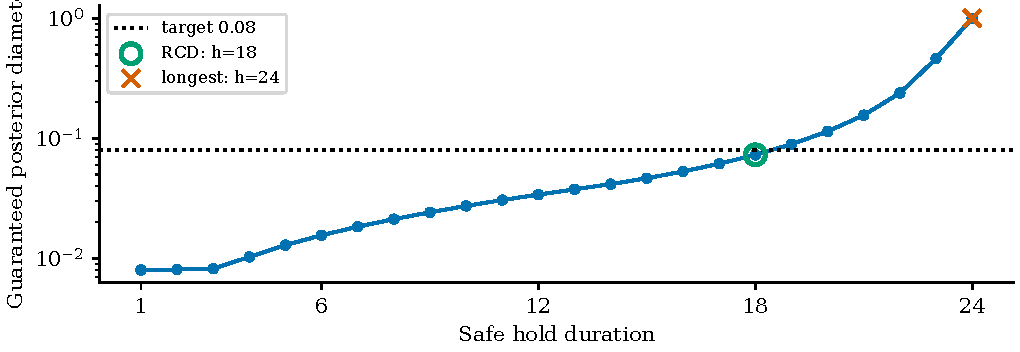
\includegraphics[width=.98\linewidth]{figures/frontier.pdf}
\caption{An exact conditional duration--resolution frontier: $A=.995R_{2\pi/24}$, $x=(.15,-.08)$, $\Theta=[.5,1.5]$, $\W=.001\mathbb B_2$, $U=.25$, and $\X=\mathbb B_2$. All 24 durations are feasible. The longest hold has poor endpoint resolution; the longest hold meeting diameter $.08$ is shorter. Values are deterministic certificate calculations, not sampled performance.}\label{fig:frontier}
\end{figure}

\begin{algorithm}[H]
\begin{minipage}{.98\linewidth}
\textbf{Input:} Observed state $x$, prior $[\ell,r]$, duration cap $H_{\max}$, target $\delta$.
\begin{enumerate}
\item Compute the prefix-safe intervals $I_h$ and scores $\kappa_h$ for all allowed durations.
\item For each nonempty $I_h$, choose its largest-magnitude endpoint $u_h$ and compute $d_h^*$.
\item If $r-\ell\le\delta$, choose the longest feasible duration. Otherwise, choose the longest duration with $d_h^*\le\delta$. If none meets the target, minimize $d_h^*$, preferring longer ties.
\item Hold $u_h$ for $h$ steps and observe the endpoint $y$.
\item Intersect the prior with the endpoint constraint~\eqref{eq:post}. Record an inconsistency if the intersection is empty.
\end{enumerate}
\end{minipage}
\caption{Resolution-constrained dwell for endpoint-only identification}\label{alg:rcd}
\end{algorithm}

The endpoint update is also explicit. Set $z_y=y-A^hx$, $v=u q_h$, and, for $v\ne0$,
\begin{equation}\label{eq:inverse}
 \widehat\theta=\frac{z_y^\top v}{v^\top v},\quad
 z_\perp=z_y-\widehat\theta v,\quad
 \Theta^+=\Theta\cap\left[\widehat\theta-\frac{\sqrt{\rho_h^2-\norm{z_\perp}^2}}{\norm{v}},\ 
 \widehat\theta+\frac{\sqrt{\rho_h^2-\norm{z_\perp}^2}}{\norm{v}}\right].
\end{equation}
A negative radicand beyond numerical tolerance or an empty intersection records model inconsistency. If $v=0$, a compatible endpoint leaves the prior unchanged. These checks are operationally important: an estimator must not silently replace incompatible data with a narrow confidence interval.


Central symmetry is essential to the simple gauge expression. For general nonsymmetric $\W$, the diameter upper bound uses the difference body $\W_h-\W_h$, but a centered noiseless endpoint need not attain its longest chord. The present theorem assumes symmetry explicitly. Nonempty interior makes the gauge finite in every direction; $q_h=0$ is handled by the zero-score convention. If $D=0$, no gain identification is needed.

For a polyhedral $\W=\{w:Cw\le d\}$, support values in~\eqref{eq:poly} are linear programs. A gauge of $\W_h$ can be computed by minimizing $s\ge0$ over $z_0,\ldots,z_{h-1}$ subject to
\[
 \sum_{i=0}^{h-1}A^iz_i=q_h,\qquad Cz_i\le s d.
\]
For a box disturbance $\W=\eta[-1,1]^n$, write $G_h=\eta[I,A,\ldots,A^{h-1}]$. The gauge is the optimum of
$\min s$ subject to $G_hz=q_h$, $-s\mathbf1\le z\le s\mathbf1$, $s\ge0$. The independent tests solve 100 such problems for random three-dimensional matrices and verify~\eqref{eq:ceiling}. No scaled-orthogonal assumption is used in that check.

To see why robust prefix safety does not require rectangularizing the unknown gain, consider any particular prefix and state inequality. Its worst case is computed with one fixed gain endpoint and an admissible sequence of disturbances. If that inequality can fail, there is a full hold with that same gain in which safety fails. Conversely, if every prefix inclusion is satisfied for both gain endpoints, every fixed intermediate gain is safe throughout the hold. Different worst-case prefixes may use different witnesses; the universal quantifier over all holds makes these separate necessary-and-sufficient tests valid.

The adaptive ambiguity floor in Proposition~\ref{prop:floor} concerns worst-case identification, even with continuous access to discrete-time states. It does not contradict consistency under independent random disturbances. In the latter model, the exact set-membership interval may shrink as rare near-boundary disturbance realizations are observed. Averaging or shrinking that interval requires a stochastic assumption to support a rate claim; we make none for the adversarial model.

\section{Constructing the adversarial endpoint regime}\label{app:adversary}
For a selected hold, let $m$ be the current prior midpoint and let
$v=(\theta-m)u q_h$. If $v\ne0$, put $e=v/\norm{v}$ and
$\alpha=\min\{1,\norm{v}/\rho_h\}$. For $A=aQ$, choose
\[
 w_{t+j}=-\eta\alpha(Q^\top)^{h-1-j}e,\qquad j=0,\ldots,h-1.
\]
Every disturbance has norm at most $\eta$. Its endpoint sum is
$-\alpha\rho_he$. This follows from the identity
\[A^{h-1-j}(Q^\top)^{h-1-j}=a^{h-1-j}I.\]
Thus the endpoint moves toward the midpoint-gain endpoint by the largest available radial amount, reaching it when possible. If $v=0$, choose zero disturbances. This construction assumes an adversary knows the actual gain, prior, and selected hold; that is allowed by the deterministic uncertainty model. It is not an estimate of the frequency of such events in industry.

The physical-state archive stores every intermediate state and actual disturbance for both regimes. The endpoint archive separately stores duration, command, prior endpoints after the update, observed norm, and certified diameter. These files allow safety, model compliance, and learning claims to be checked separately; retaining only a mean episode reward would not suffice.

\section{Full adversarial outcomes and metric definitions}\label{app:results}
\begin{table}[H]
\centering\small
\caption{Adversarial endpoint regime, 50 seeds per plant and rule. These are policy-dependent disturbance sequences, not paired random-noise estimates. Columns have the same meanings as Table~\ref{tab:main}.}
\begin{tabular}{llrrr}
\toprule
Plant & Rule & Diameter & Observations & Time resolved \\
\midrule
rotation8 & Longest & $0.30318\pm0.00000$ & 10.0 & 0.000 \\
rotation8 & Fixed-6 & $0.02591\pm0.00000$ & 40.0 & 0.975 \\
rotation8 & One-step & $0.00800\pm0.00000$ & 240.0 & 0.996 \\
rotation8 & Minimax & $0.00800\pm0.00000$ & 11.0 & 0.996 \\
rotation8 & Gaussian proxy & $0.00994\pm0.00000$ & 80.0 & 0.987 \\
rotation8 & RCD & $0.00994\pm0.00000$ & 11.0 & 0.912 \\
\midrule
rotation24 & Longest & $0.88514\pm0.03063$ & 10.0 & 0.000 \\
rotation24 & Fixed-6 & $0.00897\pm0.00025$ & 40.0 & 0.975 \\
rotation24 & One-step & $0.00800\pm0.00000$ & 240.0 & 0.996 \\
rotation24 & Minimax & $0.00800\pm0.00000$ & 11.0 & 0.996 \\
rotation24 & Gaussian proxy & $0.00820\pm0.00017$ & 40.9 & 0.987 \\
rotation24 & RCD & $0.00925\pm0.00078$ & 11.0 & 0.924 \\
\midrule
nonoscillatory & Longest & $0.02035\pm0.00497$ & 10.0 & 0.900 \\
nonoscillatory & Fixed-6 & $0.00802\pm0.00008$ & 40.0 & 0.975 \\
nonoscillatory & One-step & $0.00800\pm0.00000$ & 240.0 & 0.996 \\
nonoscillatory & Minimax & $0.00800\pm0.00000$ & 11.0 & 0.990 \\
nonoscillatory & Gaussian proxy & $0.00800\pm0.00000$ & 30.2 & 0.987 \\
nonoscillatory & RCD & $0.02035\pm0.00497$ & 10.0 & 0.900 \\
\midrule
mixed3d & Longest & $0.03036\pm0.00407$ & 10.0 & 0.900 \\
mixed3d & Fixed-6 & $0.01175\pm0.00000$ & 40.0 & 0.975 \\
mixed3d & One-step & $0.00800\pm0.00000$ & 240.0 & 0.996 \\
mixed3d & Minimax & $0.00800\pm0.00000$ & 11.0 & 0.996 \\
mixed3d & Gaussian proxy & $0.00825\pm0.00024$ & 56.0 & 0.987 \\
mixed3d & RCD & $0.03036\pm0.00407$ & 10.0 & 0.900 \\
\bottomrule
\end{tabular}
\end{table}

\begin{figure}[H]
\centering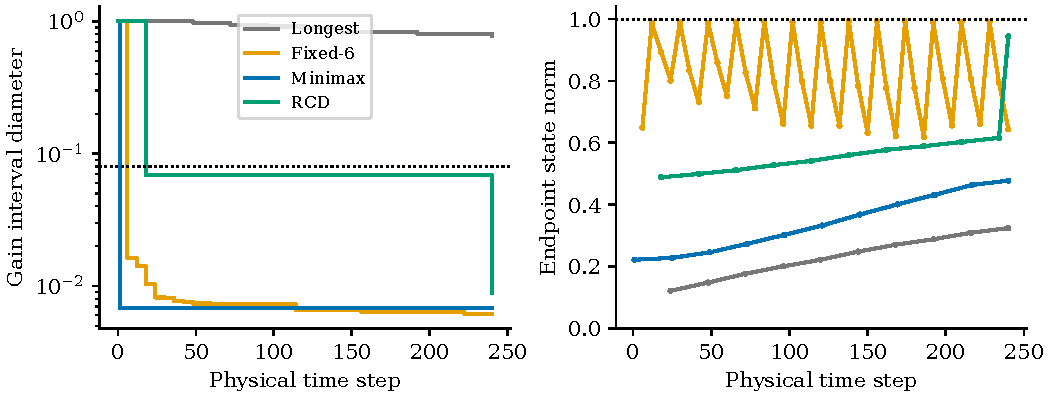
\includegraphics[width=.98\linewidth]{figures/trace.pdf}
\caption{A retained example (Rotation-24, random disturbances, seed 1000). Left: uncertainty changes only when an endpoint is observed. Right: observed state norms. Safety was additionally checked at every physical step for every run; endpoint plots alone would not establish that property.}\label{fig:trace}
\end{figure}

The first-resolution time is the first endpoint time at which the interval width is at most $.08$; episodes not resolving by step 240 are coded as 241 and are explicitly right censored. ``Time resolved'' counts a physical step only when the interval known \emph{before} that step meets the target. Observation counts exclude the initial observed state and include the final endpoint at step 240. The last hold is truncated to the remaining physical horizon and its certificate is recomputed. Final diameter is a deterministic compatible-set width, not a confidence-interval width with a nominal probability.

The full-period score sweep contains 2,880 deterministic cases: six damping factors, $.9$, $.95$, $.98$, $.995$, $.999$, and $.9999$; four periods, 4, 8, 12, and 24; five relative frequency offsets, $-.1$, $-.05$, zero, $.05$, and $.1$; and durations 1--24. The figures show selected analytic slices; the raw sweep retains every case. These calculations use a fixed input $.25$ to isolate endpoint sensitivity. State-dependent feasibility is addressed separately by the frontier and episode experiments.

\section{Matrix-error sensitivity}\label{app:mismatch}
In the model-error extension, the nominal matrix has $a=.98$, while the true radial damping is $.985$, so $\varepsilon=.005$. Period-8 and nonoscillatory plants use 50 seeds, initial norms in $[.8,.95]$, and outward disturbances. The unadjusted estimator becomes inconsistent in 50/50 and 47/50 episodes; one and three episodes, respectively, violate the safe radius before stopping. Inflating the disturbance radius to $.006$ eliminates both inconsistencies and violations in all 100 adjusted episodes. Runs stop on an empty posterior, so the unadjusted counts are not full-horizon failure probabilities. This experiment demonstrates the cost of treating a nominal model as exact, rather than suggesting that timing alone solves model uncertainty.


\section{Reproduction and audit}\label{app:reproduce}
The reference implementation uses Python, NumPy, SciPy, and Matplotlib. The tested versions are pinned in \texttt{requirements.txt}. Run
\begin{verbatim}
python3 -m unittest discover -s tests -v
python3 run_experiments.py
python3 run_mismatch.py
python3 analyze.py
python3 audit_saved.py
./build_paper.sh
\end{verbatim}
The build script sets the working directory to \texttt{paper} so that the linked L4DC class, bibliography, and figure paths resolve correctly. The local environment, elapsed time, seed range, and run count are recorded in \texttt{results/environment.json}. Timing fields can vary across reproductions and are excluded from deterministic scientific comparisons. The raw matrices, interval logic, adversarial construction, and all analysis scripts are included. The code contains no paid service calls or credential requirements.

The linked conference template on 11 October 2026 was named \texttt{L4DC2026\_template.zip}. We use its class as supplied, override the year to 2027, and leave the accepted-paper option disabled. No proceedings volume, editors, acceptance, or publication status is asserted. A named manuscript follows the supplied template's default; a different anonymization requirement would require a separate submission variant.
\end{document}
